% fig-plateleak.tex -- float wrapper for fig:plateleak.
% Data: thesis_v2/figs/fig-plateleak.json, written by thesis_v2/figs/plateleak.py from
% RESULTS_cluster/leak_crossplate.json and RESULTS_cluster/leak_sameplate.json
% (tiers.tier2_unseen_drugs.agg, *_nir_expr only).
% Placement: Sections/05-Limitations.tex, beside tab:plateleak in the "Cross-plate absolutes"
% paragraph of \section{Every result here is scoped, and the scopes differ}.
% NO width= KEY. The PDF is drawn at 142mm, which is exactly \linewidth in the body block, so
% \includegraphics{} places it at 1.0 and the 10pt type in it prints at 10pt. Adding
% [width=\linewidth] would be a silent type shrink the moment the measure changes.
\begin{figure}[htbp]
\centering
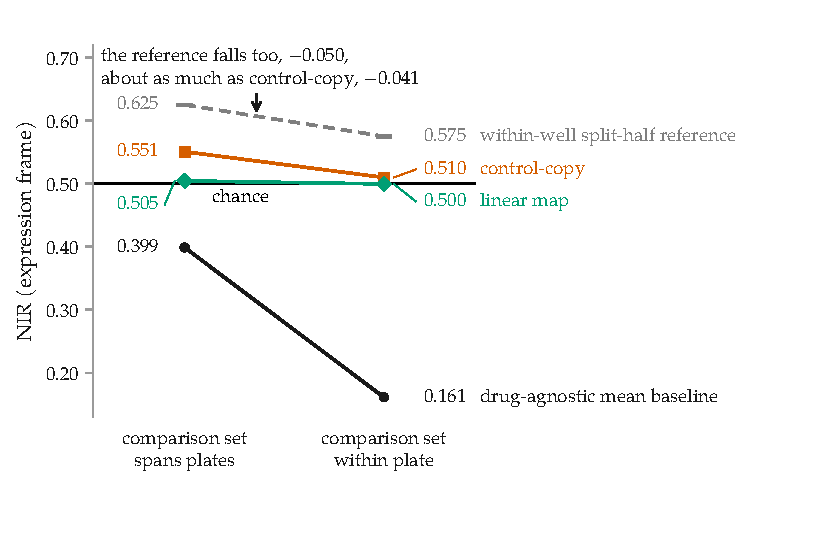
\includegraphics{fig-plateleak}
\caption[Holding the plate constant lowers the reference as well as the baseline]{%
\textbf{The batch shortcut inflates the precision reference as well as the baseline, so it is
not an offset that could be subtracted from one side of a comparison.} Expression-frame $\NIR$,
tier-2 unseen drugs, drug-agnostic arms only; the same audit as \cref{tab:plateleak}, with the
linear map read from the same block of the same two files. Forcing the comparison set within
plate collapses a mean baseline that contains no drug information whatsoever, $0.399$ to
$0.161$, and leaves control-copy close to where it was, $0.551$ to $0.510$ --- but it also
lowers the within-well split-half precision reference, $0.625$ to $0.575$, by about as much as
it lowers control-copy. That reference is the yardstick these expression-frame numbers are read
against, so the leak has no one side to be corrected on: it is a limit on what these scores may
be compared with, not an adjustable offset.
The two columns are not the same conditions. Holding the plate constant costs every condition
with no same-plate comparison set, so the within-plate column is a \emph{subset} --- $n = 998$
scored conditions, $46$ drugs, $41$ cell lines --- of the cross-plate column's
$n = \num{1163}$, $50$ drugs and $43$ cell lines, and each segment joins two scorings of
overlapping but unequal populations rather than one set of conditions rescored.
The marks are bare because neither source file carries any interval for these quantities ---
each entry is a value and its $n$ --- and this document draws only $95\%$ bootstrap intervals
clustered over cell lines. The rank-frame variants stored beside these values are a different
frame and are not drawn, and none of the values here may be set beside a residual-frame
number.}
\label{fig:plateleak}
\end{figure}
